%!TEX root = ULL_thesis_template.tex 
\chapter{Concurrent Design of the Monopode System}
\label{chapter5}

The workflow for creating a mechanical system and associated control strategy is often sequential. Typically, the mechanical and electrical hardware are developed, creating a set of confinements for the controller to be designed from. However, the mechanical/electrical system description is not always a simple one, and generating a controller for it might be unnecessarily challenging. Allowing the mechanical/electrical parameters of the system, and therefore the system's description, to be changeable could be valuable. This would allow for optimization of the complete system rather than optimizing the mechanical/electrical elements and control in isolation. Designing the system and control input in unison has been researched and is often referred to as concurrent design. This strategy has been used to develop better performing mechatronics systems \cite{Li2001}. More recent work has used advanced methods such as evolutionary strategies to select robot design parameters \cite{Wang2019}. In addition to evolutionary strategies, reinforcement learning has been shown to be a viable solution for concurrent design of 2D simulated locomotive systems \cite{Ha2019j}. This is further shown to be a viable method by demonstrating more complex morphology modifications in 3D reaching and locomotive tasks \cite{Schaff2019e}. However, these techniques have not yet been applied to flexible systems for locomotive tasks. In this chapter, a concurrent design architecture is proposed to find an optimal design and controller for the monopode jumping system defined in Chapter~\ref{chapter2}. 
%-----------------------------------------------------
\section{Concurrent Design Architecture}
\label{sec:concurrent_des_arch}
% 
\begin{figure}[tb!]
  \centering
  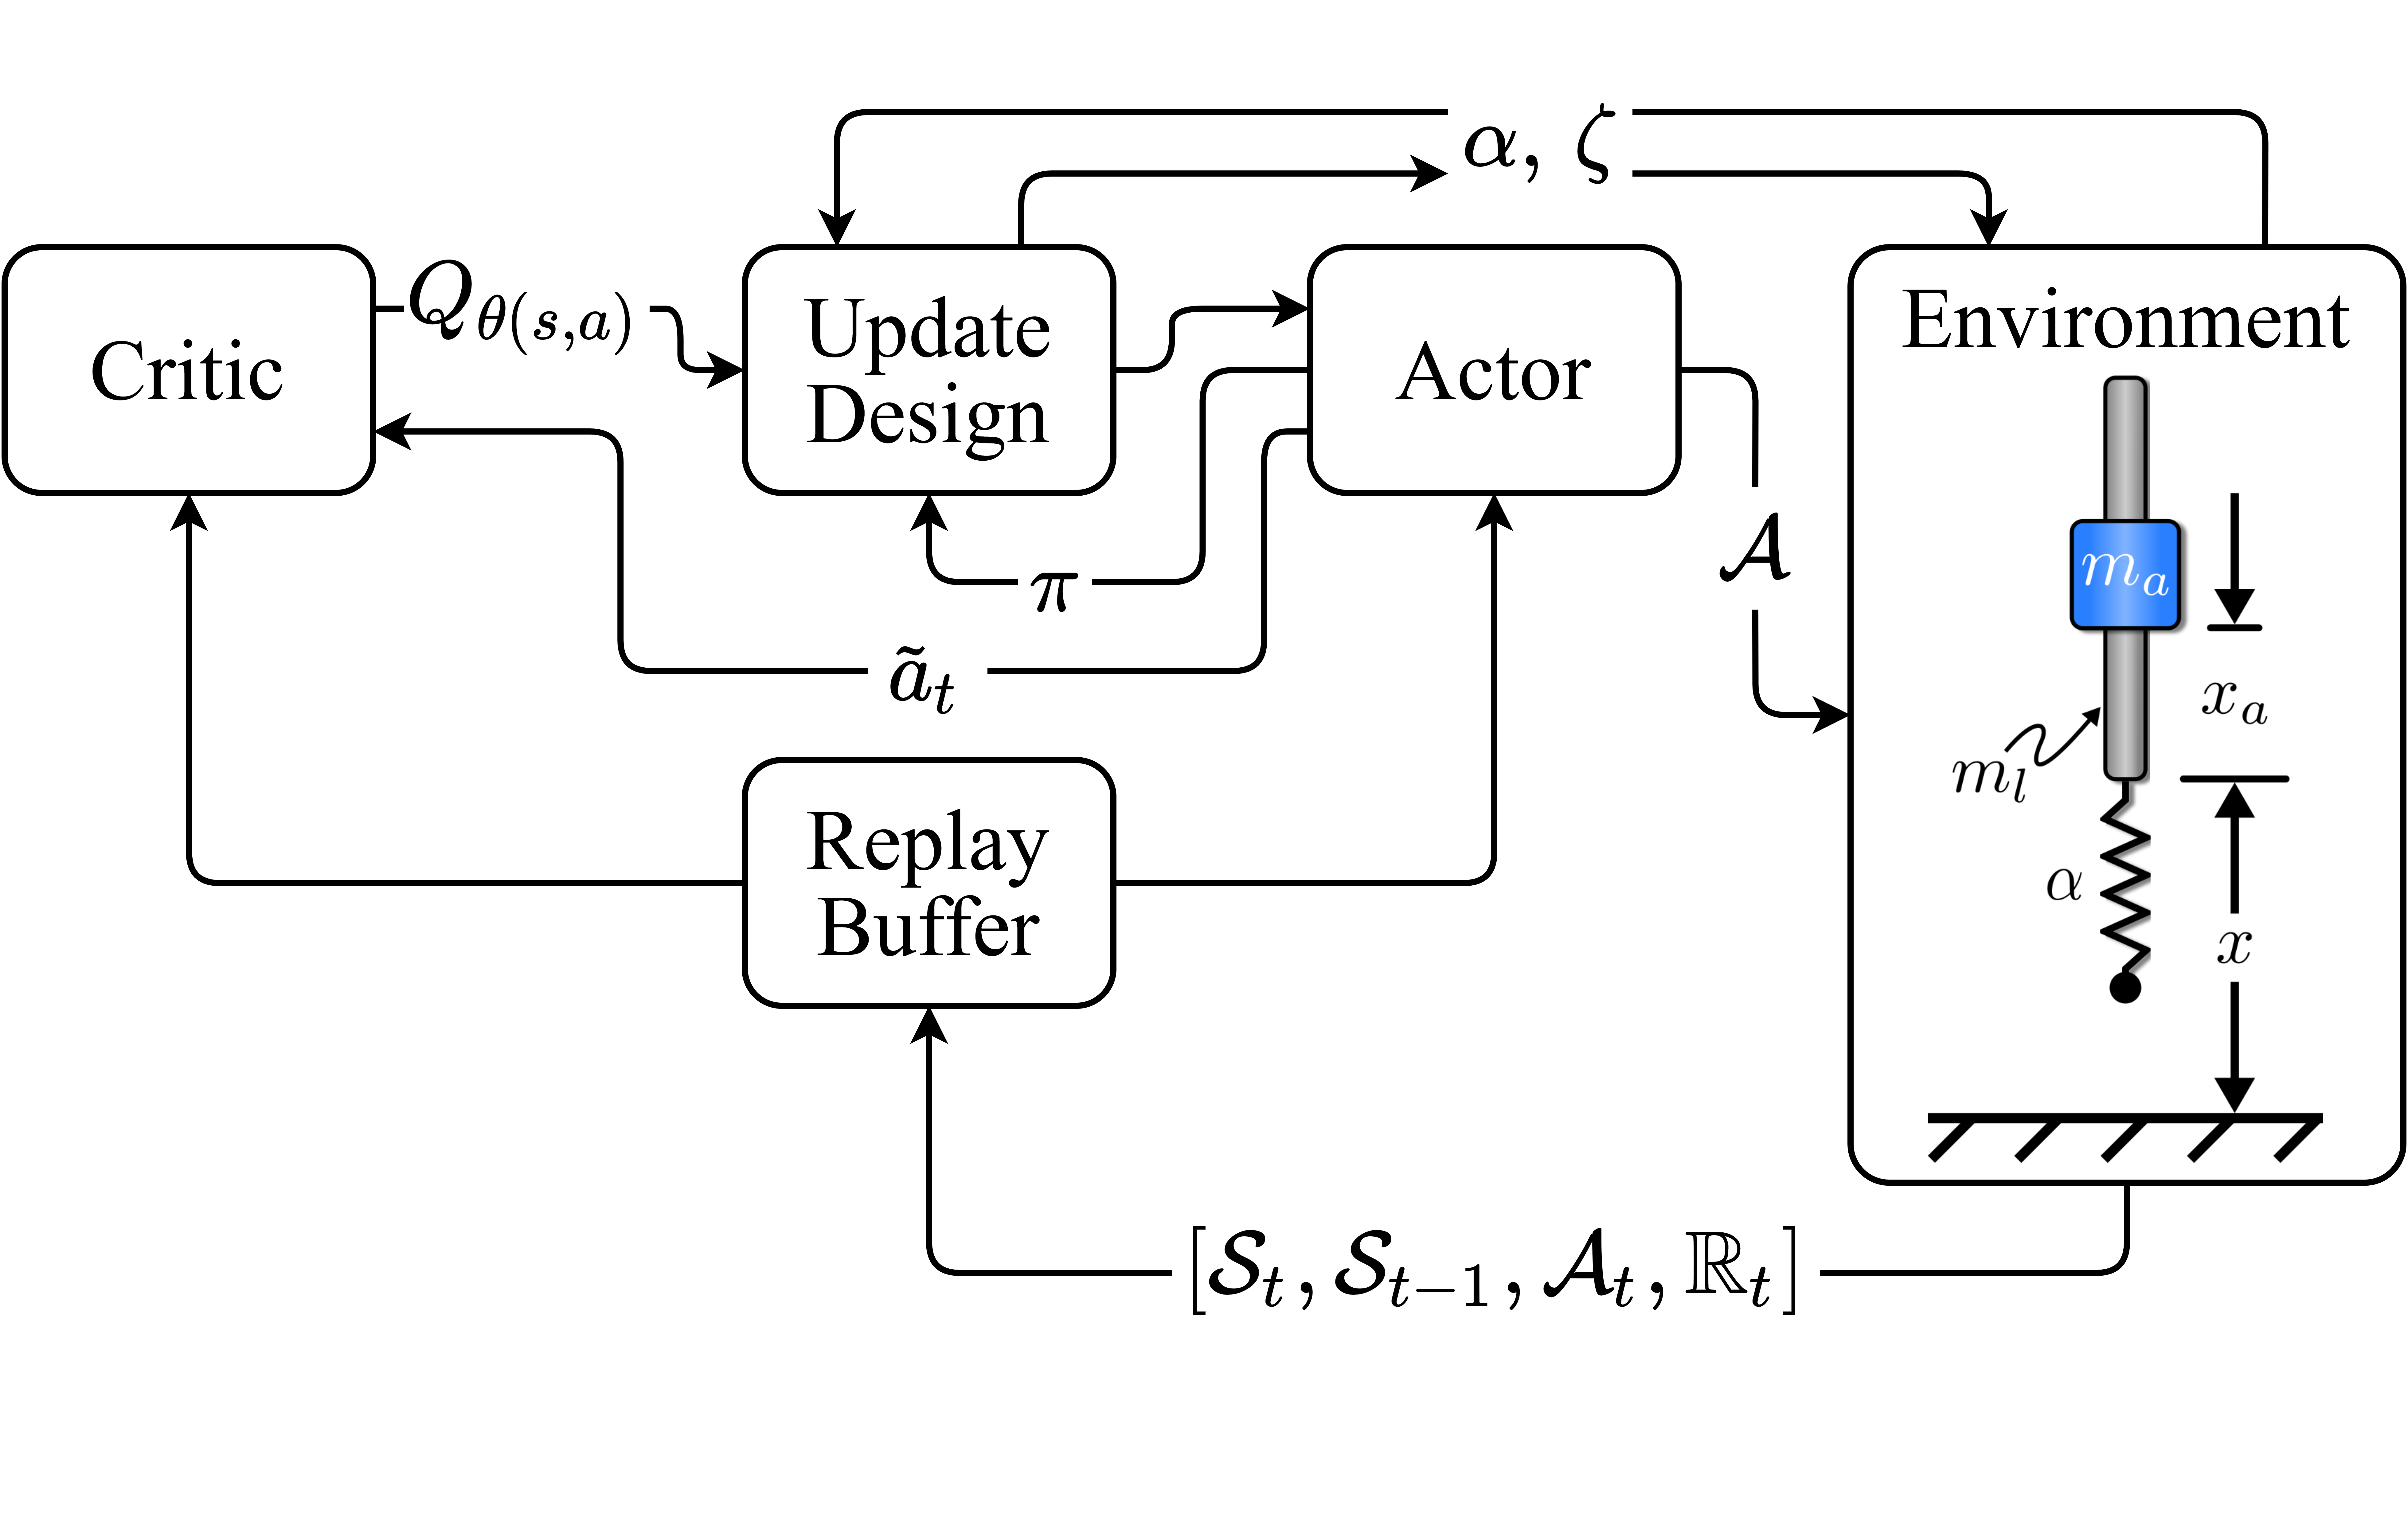
\includegraphics[width=\textwidth]{figures/Ch5/conc_des_diagram.drawio.png}  
  \caption{Concurrent Design Architecture}
  \label{fig:conc_des_diagram}
\end{figure}
% 

To define a concurrent design process utilizing RL, the proposed algorithm uses two instances of the TD3 algorithm, creating an inner and an outer loop. The first instance, which is responsible for learning the control policy, will be instantiated in a similar fashion to the what was seen in Chapter~\ref{chapter2}. It is the outer loop of the concurrent design process. The second instance, which is responsible for learning the mechanical design, is instantiated in the inner loop and in a similar fashion to what was seen in Chapter~\ref{chapter4}. A key aspect of the inner loop instantiation is that rather than using a pre-defined control input, like what was shown in Chapter~\ref{chapter4}, the simulation used the input that was being trained by the outer loop instantiation. Figure~\ref{fig:conc_des_diagram} shows the general flow of information for the concurrent design algorithm. The inner loop, replicating the work from Chapter~\ref{chapter4}, is within the ``Update Design'' block. The description of the inner loop was shown in Figure~\ref{fig:TD3_mech_design}, only the defined input that was used in Chapter~\ref{chapter4} was replaced in this diagram by the current policy, $\pi$. A detailed algorithm, describing the process presented in Figure~\ref{fig:conc_des_diagram}, is presented in Appendix~\ref{app:concurrent_des_algo}. 

%-----------------------------------------------------
\section{Mechanical Design Update}
\subsection{Discrete vs. continuous}
As is further discussed in Appendix~\ref{app:concurrent_des_algo}, there are two different methods for implementing the inner loop of the concurrent design algorithm. The first is called the \textit{discrete} method, where at each environment design update, the model learning the design is instantiated fresh and learns a design from scratch. The second method is called \textit{continuous}, where at each environment update the model learning the design is saved and reloaded so that the model that is learning a design is the same over the course of the controller model training. 

\subsection{Averaging design policies}
In Chapter~\ref{chapter4}, average designs found from 50 different policies were shown, and it was seen that design choice can vary between policies, depending on factors such as the reward the policy receives and the design space limits. To replicate the results in Chapter~\ref{chapter4}, and to ensure that the mechanical design inner loop did not suffer from a single policy finding a locally optimal design, $n$ design policies were instantiated at each design update. The average design found was used to update the environment within the outer loop. This methodology was applied to both the discrete and the continuous methods of the mechanical design update. In this work, $n$ was set as five as it proved to resolve one of the policies finding a design which strayed from the average design.

\subsection{Differing reward types}
Depending on the reward passed to the design update inner loop, the performance of the control policy may immediately increase or decrease when the design is updated. For example, if the rewards for both inner and outer loops reward the same metric, the control policy within the outer loop should see an increase in performance after a design update. If, however, the rewards for the inner and outer loops differ, where the outer loop might reward height, for example, and the inner rewards efficiency, the control policy may experience an immediate decrease in performance after a design update. Utilizing differing rewards might serve as a tool to generate designs where, as suggested, the control policy is defined to accomplish a task and the design is optimized to allow the control policy to do that task efficiently. 

\subsection{Design update rate}
When the inner loop makes an update to the environment that the policy within the outer loop is being trained on, the policy should see an immediate performance change. These step-like changes are likely to result in a policy learning less data efficiently. Because of this, a new hyperparameter is introduced, which is the rate at which the design is updated. As is shown in Appendix~\ref{app:concurrent_des_algo}, the design is updated in line with the control policy but not at the same rate. Regardless, the design update rate is directly tied to the policy update. It is suggested that for this architecture the design is updated every $\delta$ policy updates where $\delta$ depends on the complexity of the control policy being trained. For more complex control policies, where the learning process might require more environment interactions to learn, $\delta$ should be set to a higher value so that the control policy can learn a design without the added difficulty of dynamic environment design parameters.

\subsection{Design space limitations}
The work shown in Chapter~\ref{chapter4} discussed two design spaces, both with differing nominal values as well as upper and lower limits. This raises the concern of design space choice for the concurrent design architecture. It was shown in Chapter~\ref{chapter4}, that the design space had an effect on the final designs learned, both in terms of the number of iterations required to converge, and in variance seen across network initializations. In the work presented in this chapter, the design space nominal values and limits were chosen to partially replicate the work in Chapter~\ref{chapter4}. Regarding the spring constant, the nominal value used was what was presented in Table~\ref{tab:monopode_params}, with the limits being set to $\pm$90\% of the nominal value. As for the damping ratio, since it was shown to have learned extremely low damping ratios in most learning cases, the design space was set as a range from 0 to 0.01. 

%-----------------------------------------------------
\section{Environment Definition}
\subsection{Learning the controller}
The outer loop of the concurrent design architecture was defined similar to what was shown in Chapter~\ref{chapter2}, where a traditional RL environment aligning with the standards set by OpenAI for a Gym environment was created \cite{Brockman2016c}. The monopode, also described in Section~\ref{sec:monopode}, was used to define the environment and evaluate the methods discussed in this chapter. The action applied to the environment and observation saved to the replay buffer were defined, respectively, as follows:
% 
\begin{equation}
  \begin{aligned}
      \mathcal{A} = [\ddot{x}_{a_t}]
  \end{aligned}
\end{equation}
% 
\begin{equation}
  \begin{aligned}
    \mathcal{S} = \left[ x_{a_t}, \dot{x}_{a_t}, x_t, \dot{x}_t \right]
  \end{aligned}
\end{equation}
% 
where $x_t$ and $\dot{x}_t$ were the position and velocity of the monopode at time $t$, and $x_{a_t}$, $\dot{x}_{a_t}$ and $\ddot{x}_{a_t}$ were the position, velocity and acceleration of the actuator, respectively. The observation space was defined as:

Differing from the evaluation completed in Chapter~\ref{chapter2}, only the stutter jumping command was evaluated. Therefore, the stopping conditions for the environment were either the monopode completing two jumps or the time step limit. For this work, the time step limit was set to 400 steps at 0.01 seconds per step. Additional information regarding the stutter jump command was provided in Section~\ref{sec:monopode}. The values of the nominal constants of the monopode were shown in Table~\ref{tab:monopode_params} within Section~\ref{sec:monopode}.

\subsection{Learning the design}
To allow the inner loop RL algorithm to find a mechanical design within the outer control loop, a second reinforcement learning environment was defined, again conforming to the OpenAI Gym standard \cite{Brockman2016c}, in a similar fashion to what was discussed in Chapter~\ref{chapter4}. Differing from Chapter~\ref{chapter4}, however, the control input, rather than being fixed, is captured from the outer loop and used to evaluate the performance of different design choices. The mechanical parameters the algorithm was tasked with optimizing were the spring constant and the damping ratio of the monopode jumping system.

At each episode during training, the policy of the algorithm selected a set of design parameters from a distribution of predefined parameter ranges and saved the timeseries simulation information in the replay buffer. The actions applied, $\mathcal{A}$, within the environment were the designs selected and were defined as follows:
% 
\begin{equation}
    \begin{aligned}
    \mathcal{A} = \{ \{ a_{\alpha} \in \mathbb{R}: [0.1 \alpha, 1.9 \alpha] \}, \, \{ a_{\zeta} \in \mathbb{R}: [0, 0.01] \} \}
    \end{aligned}
\end{equation}
% 
where $\alpha$ is the nominal spring constant of the monopode, $x_t$ and $\dot{x}_t$ are the rod height and velocity steps of the monopode, and $x_{a_t}$ and $\dot{x}_{a_t}$ are the actuator position and velocity steps of the monopode, all captured during simulation. The nominal values of the constants were shown in Table~\ref{tab:monopode_params} within Section~\ref{sec:monopode}. The transitions saved, were the timeseries information, and were defined as:
% 
\begin{equation}
  \begin{aligned}
    \mathcal{S}= \{ \textup{\textbf{X}}, \dot{\textup{\textbf{X}}}, \textup{\textbf{X}}_a, \dot{\textup{\textbf{X}}}_a \}
  \end{aligned}
\end{equation}
% 
where $\textup{\textbf{X}}$, $\dot{\textup{\textbf{X}}}$, $\textup{\textbf{X}}_a$ and $\dot{\textup{\textbf{X}}}_a$ are vectors of time evolution for the position and velocity of the rod and the position and velocity of the actuator, respectively.

%-----------------------------------------------------
\section{Deploying the Algorithm}
As is discussed in Section~\ref{sec:concurrent_des_arch}, an inner and outer instantiation of the TD3 algorithm are generated to create the concurrent design architecture. Similar to what was practiced in previous chapters, multiple instances of the algorithm were run to evaluate the ability of the architecture to perform with different network initializations. Ten total instances were evaluated so that average performance data could be collected.

The outer loop was instantiated in a similar fashion as to what was discussed in Chapter~\ref{chapter2}, except that the number of total training steps was increased from 500k to 750k. This was done as the control policy was anticipated to be more difficult to learn given the parameters of the environment would be changing due to the inner loop. The training hyperparameters used for the outer loop instantiation of the TD3 algorithm are presented in Table~\ref{tab:conc_ctr_hyperparams}.

\begin{table}[tb!]
  \caption{Outer Loop TD3 Training Hyperparameters}
  \begin{center}
  \vspace{-12pt}
  \begin{tabular}{c c}
  \textbf{Hyperameter}            & \textbf{Value}                  \\
  \hline
  \hline
  Learning Rate, $\alpha$         & 0.001                           \\
  Learning Starts                 & 1000 Steps                      \\
  Batch Size                      & 100 Transitions                 \\
  Tau, $\tau$                     & 0.005                           \\
  Gamma, $\gamma$                 & 0.99                            \\
  Training Frequency              & 1:Episode                       \\
  Gradient Steps                  & $\propto$ Training Frequency    \\
  Action Noise,  $\epsilon$       & None                            \\
  Policy Delay                    & 1 : 2 Q-Function Updates        \\
  Target Policy Noise, $\epsilon$ & 0.2                             \\
  Target Policy Clip, $c$         & 0.5                             \\
  Seed                            & 5 Random Seeds                 \\
  \hline
  \hline
  \end{tabular}
  \label{tab:conc_ctr_hyperparams}
  \end{center}
\end{table}

\begin{table}[tb!]
  \caption{TD3 Training Hyperparameters}
  \begin{center}
  \vspace{-12pt}
  \begin{tabular}{c c}
  \textbf{Hyperameter}            & \textbf{Value}                  \\
  \hline
  \hline
  Learning Rate, $\alpha$         & 0.001                           \\
  Learning Starts                 & 100 Steps                       \\
  Batch Size                      & 100 Transitions                 \\
  Tau, $\tau$                     & 0.005                           \\
  Gamma, $\gamma$                 & 0.99                            \\
  Training Frequency              & 1:Episode                       \\
  Gradient Steps                  & $\propto$ Training Frequency    \\
  Action Noise,  $\epsilon$       & None                            \\
  Policy Delay                    & 1 : 2 Q-Function Updates        \\
  Target Policy Noise, $\epsilon$ & 0.2                             \\
  Target Policy Clip, $c$         & 0.5                             \\
  Seed                            & 5 Random Seeds                \\
  \hline
  \hline
  \end{tabular}
  \label{tab:conc_mech_hyperparams}
  \end{center}
\end{table}

The inner loop, was instantiated in a similar fashion to what is shown in Chapter~\ref{chapter4}. This instantiation of the TD3 algorithm was created within the outer instantiation of the TD3 algorithm, using the policy being trained within the outer loop to optimize the environment used in the outer loop. The number of training steps taken by each instantiation was 1000, to best replicate the results from Chapter~\ref{chapter4}. Additional hyperparameters used for each of the five instantiations of the inner TD3 algorithm are presented in Table~\ref{tab:conc_mech_hyperparams}.

%-----------------------------------------------------
\section{Discrete vs Continuous Designs}
\label{sec:disc_vs_cont}
%  
\begin{figure}[tb!]
  \centering
  \begin{subfigure}{.49\textwidth}
          \centering
          \includegraphics[width=\textwidth]{figures/Ch5/dis_vs_cont/avg_eff_rew_.png}  
          \caption{Reward During Training for Efficient Design}
          \label{fig:disc_vs_cont_rew_eff}
  \end{subfigure}%
  \hfill
  \begin{subfigure}{.49\textwidth}
          \centering
          \includegraphics[width=\textwidth]{figures/Ch5/dis_vs_cont/avg_hei_rew_.png}  
          \caption{Reward During Training for Height Design}
          \label{fig:disc_vs_cont_rew_high}
  \end{subfigure}
   \caption{Reward During Training for Discrete and Continuous Implementation Methods of Concurrent Design}
   \label{fig:disc_vs_cont_rew}
\end{figure}
% 

\subsection{Reward vs learning step}

Figure~\ref{fig:disc_vs_cont_rew} shows the reward received during training for the high and efficient jumping strategies comparing the discrete and continuous implementations. The rewards can be used to evaluate the learning differences between the discrete and continuous methods used to define a concurrent design architecture. The design update rate for this evaluation was set to 1000 for both methods. Figure~\ref{fig:disc_vs_cont_rew_eff}, comparing the rewards during training for the efficient jumping control strategies show little difference between the two methods. Both the design architecture display rapid learning capabilities similar to what was shown for the efficient controller types in Chapter~\ref{chapter2}.

Figure~\ref{fig:disc_vs_cont_rew_high}, comparing the rewards during training for the high jumping design architecture, show some differences between the two methods. The discrete method learns a higher performing policy and one that is less susceptible to performance loss due to an over-fitting design policy towards the end of training. Both methods, however, have policies that are losing rewards due to over fitting towards the end of training.

\subsection{Designs learned}
%  
\begin{figure}[tb!]
  \centering
  \begin{subfigure}{.49\textwidth}
          \centering
          \includegraphics[width=\textwidth]{figures/Ch5/dis_vs_cont/avg_eff_spring_.png}  
          \caption{Spring Constant Learned During Training for Efficient Design}
          \label{fig:disc_vs_cont_spring_eff}
  \end{subfigure}%
  \hfill
  \begin{subfigure}{.49\textwidth}
          \centering
          \includegraphics[width=\textwidth]{figures/Ch5/dis_vs_cont/avg_hei_spring_.png}  
          \caption{Spring Constant Learned During Training for Height Design}
          \label{fig:disc_vs_cont_spring_high}
  \end{subfigure}
   \caption{Spring Constant During Training for Discrete and Continuous Implementation Methods of Concurrent Design}
   \label{fig:disc_vs_cont_spring}
\end{figure}
% 

Figure~\ref{fig:disc_vs_cont_spring} shows the learning of the spring constant for the efficient and high jumping concurrent design types. These can be used to evaluate the differences in the learned designs between the discrete and the continuous mechanical update methods. It is apparent that the learning of the designs for both jumping cases is more continuous for the continuous design update method, where the policy for learning a design is retained. In both jumping cases, the continuous method learns higher spring rates on average across different instantiations of the concurrent design architecture. This is likely because higher spring rates create higher jumps for poorly trained policies which are learned early in training. For the continuous update method, the learned designs have a greater effect throughout the entirety of the learning process. Furthermore, there are obvious differences between the methods regarding standard deviation across outer loop instantiations, where the continuous method has much less deviation. This does not directly translate to performance consistency, since each instantiation of the control policy will have its own design. It does, however, show that across different concurrent design instantiations, the continuous method converges to a more consistent design.

%  
\begin{figure}[tb!]
  \centering
  \begin{subfigure}{.49\textwidth}
          \centering
          \includegraphics[width=\textwidth]{figures/Ch5/dis_vs_cont/avg_eff_zeta_.png}  
          \caption{Damping Ratio Learned During Training for Efficient Design}
          \label{fig:disc_vs_cont_zeta_eff}
  \end{subfigure}%
  \hfill
  \begin{subfigure}{.49\textwidth}
          \centering
          \includegraphics[width=\textwidth]{figures/Ch5/dis_vs_cont/avg_hei_zeta_.png}  
          \caption{Damping Ratio Learned During Training for Height Design}
          \label{fig:disc_vs_cont_zeta_high}
  \end{subfigure}
   \caption{Damping Ratio During Training for Discrete and Continuous Implementation Methods of Concurrent Design}
   \label{fig:disc_vs_cont_zeta}
\end{figure}
% 

Figure~\ref{fig:disc_vs_cont_zeta} shows the learning of the damping ratio for the efficient and high jumping concurrent design types. In both cases, the continuous method learned a lower damping ratio than the discrete method. Similar to the learning of the spring rate, the continuous method learns a design with less discrete value changes throughout the control policy training. This is particularly obvious in the case where the policy is learning a high jumping strategy. For the efficient jumping strategy, the damping ratios found across concurrent design instantiations vary greatly, as is shown by the large standard deviation among the learned ratios. Whereas, in the case of the high jumping strategy, the difference in standard deviation is lower. The increase in standard deviation of learned damping ratios is similar to the results shown in Chapter~\ref{chapter4} where changes in damping ratio were shown to be less critical than changes in spring rate.

\subsection{Resulting input and jumping performance}

Comparing the learning processes of the continuous and discrete methods, can only give some intuition regarding the differences between the methods. Each instantiation of the concurrent design process has its own learned controller and associated design. Because of this, differing designs might not have as great of an effect on final performance because the associated controller was trained for said design specifically. As such, it is necessary to evaluate the differences seen in performance between the two methods discussed. 

%  
\begin{figure}[tb!]
  \centering
  \begin{subfigure}{.49\textwidth}
    \centering
    \includegraphics[width=\textwidth]{figures/Ch5/dis_vs_cont/avg_eff_Input_.png}  
    \caption{Average Input for Efficient Concurrent Designs}
    \label{fig:disc_vs_cont_input_eff}
  \end{subfigure}%
  \hfill
  \begin{subfigure}{.49\textwidth}
    \centering
    \includegraphics[width=\textwidth]{figures/Ch5/dis_vs_cont/avg_hei_Input_.png}  
    \caption{Average Input for High Jumping Concurrent Designs}
    \label{fig:disc_vs_cont_input_hei}
  \end{subfigure}%
   \caption{Average Controller Performance for Efficient Concurrent Designs}
   \label{fig:disc_vs_cont_input}
\end{figure}
% 

Starting with the learned inputs for the efficient and high jumping designs, shown in Figure~\ref{fig:disc_vs_cont_input}, it is apparent that the learned input for the efficient jumping type is not one which would accomplish a high jump. Figure~\ref{fig:disc_vs_cont_input_eff}, showing the learned commands for the efficient jumping designs, shows that the controllers for the discrete method will accelerate in the negative direction for a short period of time and then stop for the rest of the command. As for the continuous method, across network initializations, the command directions are split such that the average is to stay stationary. This learned input is not consistent with what was shown to be learned in Chapter~\ref{chapter2}, and is likely the result of increasing the complexity of the learning process where already there existed a fragile reward function. 

The inputs for the high jumping designs are shown in Figure~\ref{fig:disc_vs_cont_input_hei}. For this jump type, the timing and magnitude of the inputs of the discrete and continuous methods are very similar throughout most of the command. However, as will be discussed later, the differences do create differing jumping performance. The largest difference between the methods, regarding the inputs learned, are towards the end of the command, where both methods result in a control policy that accelerates the actuator upwards. This resulted from the definition of the reward where the policy was trying to maximize the height at every time step. The differences in the timing seen in the final command are not entirely clear regarding how the discrete and continuous methods effected the learned command. 

%  
\begin{figure}[tb!]
  \centering
  \begin{subfigure}{.49\textwidth}
    \centering
    \includegraphics[width=\textwidth]{figures/Ch5/dis_vs_cont/avg_eff_RodPos_.png}  
    \caption{Average Jumping Performance for Efficient Concurrent Designs}
    \label{fig:disc_vs_cont_rodpos_eff}
  \end{subfigure}
  \hfill
  \begin{subfigure}{.49\textwidth}
    \centering
    \includegraphics[width=\textwidth]{figures/Ch5/dis_vs_cont/avg_hei_RodPos_.png}  
    \caption{Average Jumping Performance for High Jumping Concurrent Designs}
    \label{fig:disc_vs_cont_rodpos_hei}
  \end{subfigure}
   \caption{Average Controller Performance for High Jumping Concurrent Designs}
   \label{fig:disc_vs_cont_rodpos}
\end{figure}
% 

The average timeseries jumping performances of the efficient and high jumping strategies for the discrete and continuous methods can be seen in Figure~\ref{fig:disc_vs_cont_rodpos}. Figure~\ref{fig:disc_vs_cont_rodpos_eff} shows the jumping performance of the efficient concurrent design. It is apparent the increased complexity of the efficient command makes for a difficult policy to learn. That is, the policy cannot find a consistent control strategy that can overcome the increased complexity of a dynamic environment. The input, only accelerating in one direction for a short period of time, allows the monopode to jump just above the zero point so it can stutter bounce rather than stutter jump. A potential solution to this poorly learned policy could be to modify the reward such that it returned a normalized score to better equip the policy with usable information.

The jumping performance of the high jumping concurrent designs are shown in Figure~\ref{fig:disc_vs_cont_rodpos_hei}. The learned inputs for the discrete and continuous methods, shown in Figure~\ref{fig:disc_vs_cont_input_hei}, being similar in timing and magnitude, create similar jumping performance. The continuous method, having an input comprised of noisy commands does not store as much energy within the spring and therefore does not jump the monopode as high. Rather than storing increased energy within the spring, it instead relies on the final upward acceleration of the actuator to get to its maximum height. The discrete method, though employing the same final upward acceleration, does so later than the continuous method and therefore does not capitalize on it for achieving maximum height. Regarding the consistency across instantiations of the concurrent design architecture, the discrete methods learn concurrent designs that result in commands that more consistently jump higher. Additionally, the discrete methods leads to commands that perform better than the continuous method in the best cases.

%-----------------------------------------------------
\section{Effects of Differing Update Rate}
\label{sec:changing_ur}

In addition to discovering the differences in learning, and final design performance, due to employing the discrete/continuous method, the differences when changing the design update rate were also evaluated. The update rate value is tied to the rate that the control policy is updated in the outer loop. In the previous section, the results presented where trained using a design update rate of 1000, \textit{i.e.} the design was updated every 1000 control policy updates. It was shown that, in general, the efficient designs could not learn a concurrent design that successfully completed a stutter jumping command. It was also shown that the discrete method produced designs that more consistently resulted in high jumping performance for the high jumping strategy. As such, in this section, design update rates of 1000, 3000, and 5000 are evaluated and compared using the discrete method of mechanical design updating.

\subsection{Reward vs learning step}
%  
\begin{figure}[tb!]
  \centering
  \begin{subfigure}{.49\textwidth}
          \centering
          \includegraphics[width=\textwidth]{figures/Ch5/comp_update_rate/avg_eff_rew_.png}  
          \caption{Reward During Training for Efficient Design}
          \label{fig:comp_ur_rew_eff}
  \end{subfigure}%
  \hfill
  \begin{subfigure}{.49\textwidth}
          \centering
          \includegraphics[width=\textwidth]{figures/Ch5/comp_update_rate/avg_hei_rew_.png}  
          \caption{Reward During Training for Height Design}
          \label{fig:comp_ur_rew_high}
  \end{subfigure}
   \caption{Reward During Training for Discrete and Continuous Implementation Methods of Concurrent Design}
   \label{fig:comp_ur_rew}
\end{figure}
% 
Figure~\ref{fig:comp_ur_rew} shows the rewards during training for each of the three mechanical update rates evaluated for the high and efficient jumping strategies for the discrete update method. In the case of the efficient strategy, seen in Figure~\ref{fig:comp_ur_rew_eff}, there were little differences found when altering the update rate. However, it seems that lowering the rate at which the mechanical design is updated results in the policy drastically changing in the middle of learning. This is likely because, as discussed earlier, as the design changes, the policy will see an immediate change, and when lowering the update rate, the design changes less often and more drastically.

As for the high jumping strategies, seen in Figure~\ref{fig:comp_ur_rew_high}, there are more obvious differences. It is apparent that lowering the update rate decreases policy performance with respect to the reward received. Additionally, in the beginning of training, there is less variance in the performance of the policies across network instantiations. This is directly related to how often the mechanical design is updated and will be further explained when evaluating the mechanical designs learned. Finally, it is shown that over-fitting within the design policy becomes less apparent as the update rate decreases.   

\subsection{Designs learned}
%  
\begin{figure}[tb!]
  \centering
  \begin{subfigure}{.49\textwidth}
          \centering
          \includegraphics[width=\textwidth]{figures/Ch5/comp_update_rate/avg_eff_spring_.png}  
          \caption{Spring Constant Learned During Training for Efficient Design}
          \label{fig:comp_ur_spring_eff}
  \end{subfigure}%
  \hfill
  \begin{subfigure}{.49\textwidth}
          \centering
          \includegraphics[width=\textwidth]{figures/Ch5/comp_update_rate/avg_hei_spring_.png}  
          \caption{Spring Constant Learned During Training for Height Design}
          \label{fig:comp_ur_spring_high}
  \end{subfigure}
   \caption{Spring Constant During Training for Discrete and Continuous Implementation Methods of Concurrent Design}
   \label{fig:comp_ur_spring}
\end{figure}
% 
The learned spring constant value during training, for both the efficient and high jumping strategies, is displayed for the three different update rates being evaluated in Figure~\ref{fig:comp_ur_spring}. In both cases, the increase in update rate directly translates to an increase in rollout time before the design update policy can begin learning designs. This was shown to translate to the rewards in that the concurrent design instantiations with lower update rates required more steps to learn performant policies. 

%  
\begin{figure}[tb!]
  \centering
  \begin{subfigure}{.49\textwidth}
          \centering
          \includegraphics[width=\textwidth]{figures/Ch5/comp_update_rate/avg_eff_zeta_.png}  
          \caption{Damping Ratio Learned During Training for Efficient Design}
          \label{fig:comp_ur_zeta_eff}
  \end{subfigure}%
  \hfill
  \begin{subfigure}{.49\textwidth}
          \centering
          \includegraphics[width=\textwidth]{figures/Ch5/comp_update_rate/avg_hei_zeta_.png}  
          \caption{Damping Ratio Learned During Training for Height Design}
          \label{fig:comp_ur_zeta_high}
  \end{subfigure}
   \caption{Damping Ratio During Training for Discrete and Continuous Implementation Methods of Concurrent Design}
   \label{fig:comp_ur_zeta}
\end{figure}
% 

The learning of the damping ratios for the three different update rates being evaluating are shown in Figure~\ref{fig:comp_ur_zeta}. In the case of the efficient strategy, shown in Figure~\ref{fig:comp_ur_zeta_eff}, there is little difference outside of the increasing rollout period. As for the high jumping strategies, shown in Figure~\ref{fig:comp_ur_zeta_high}, the differences are more pronounced. Primarily, as the update rate decreases, the consistency of the designs learned throughout training increases. This can be explained in that the control policy has more time to train a high performing policy before the design changes and therefore is able to better train a controller on the most current design. 

\subsection{Resulting input and jumping performance}
%  
\begin{figure}[tb!]
  \centering
  \begin{subfigure}{.49\textwidth}
    \centering
    \includegraphics[width=\textwidth]{figures/Ch5/comp_update_rate/avg_eff_Input_.png}  
    \caption{Average Input for Efficient Concurrent Designs}
    \label{fig:comp_ur_input_eff}
  \end{subfigure}%
  \hfill
  \begin{subfigure}{.49\textwidth}
    \centering
    \includegraphics[width=\textwidth]{figures/Ch5/comp_update_rate/avg_hei_Input_.png}  
    \caption{Average Input for High Jumping Concurrent Designs}
    \label{fig:comp_ur_input_hei}
  \end{subfigure}%
   \caption{Average Controller Performance for Efficient Concurrent Designs}
   \label{fig:comp_ur_input}
\end{figure}
% 

Average learned input for the efficient and high jumping concurrent designs for the three different update rates evaluated are shown in Figure~\ref{fig:comp_ur_input}. There are clear differences regarding the policies learned across the different design update rates. For the efficient jumping strategy, shown in Figure~\ref{fig:comp_ur_input_eff}, reducing the rate that the design is updated allows the policies to learn a strategy beyond a single bang command. The lower update rates also caused the policies to learn an input that accelerated the actuator in the opposite direction for the initial acceleration. Additionally, for the middle update rate evaluated, where the design was updated every 3000 policy updates, the policy for one of the 5 instantiations learned a command that performed what would be considered a stutter jump. This inconsistency might be solved by either generating a more stable reward condition, or by better tuning the learning hyperparameters within the inner/outer loops. Regardless, the differences in input shapes show that changes in update rate can have an impact on learned policies. 

Figure~\ref{fig:comp_ur_input_hei} shows the inputs learned for the high jumping concurrent designs. Similar to the inputs learned for the efficient concurrent designs, there are differences that can be seen both in timing and magnitude between the different update rates evaluated. In both the 1:3k and the 1:5k update rates, the average commands learned have higher magnitude accelerations in the positive direction and in the last negative direction. Additionally, these update rates produce commands that, like the lower update rates for the efficient concurrent designs, accelerate in the positive direction for the initial acceleration command. Finally, the commands with lower update rates learn more consistent commands across different instantiations of the concurrent design architecture. 

%  
\begin{figure}[tb!]
  \centering
  \begin{subfigure}{.49\textwidth}
    \centering
    \includegraphics[width=\textwidth]{figures/Ch5/comp_update_rate/avg_eff_RodPos_.png}  
    \caption{Average Jumping Performance for Efficient Concurrent Designs}
    \label{fig:comp_ur_rodpos_eff}
  \end{subfigure}
  \hfill
  \begin{subfigure}{.49\textwidth}
    \centering
    \includegraphics[width=\textwidth]{figures/Ch5/comp_update_rate/avg_hei_RodPos_.png}  
    \caption{Average Jumping Performance for High Jumping Concurrent Designs}
    \label{fig:comp_ur_rodpos_hei}
  \end{subfigure}
   \caption{Average Controller Performance for High Jumping Concurrent Designs}
   \label{fig:comp_ur_rodpos}
\end{figure}
% 

Average jumping performance resulting from the learned input for the efficient and high jumping strategies for the three different update rates evaluated are shown in Figure~\ref{fig:comp_ur_rodpos}. Figure~\ref{fig:comp_ur_rodpos_eff}, showing the resulting jumping performance from the efficient command input, shows the effects of the differing inputs. Firstly, looking at the performance of the 1:3k update rate, it is clear that changes to the update rate can result in a policy that learned a design to accomplish a stutter jump. However, as was pointed out in the input discussion, this behavior is highly inconsistent and exists within a set of commands that are already inconsistent in general. Regardless, the effects of the different input directions can be seen in that the lower update rate learned concurrent designs do learn to initially compress the spring to create the energy to jump. It appears, however, that the rewards punish power in a way that forces the commands not to learn to fully complete a stutter jump, as they rely too much on the spring energy alone to complete the jumping commands.

Figure~\ref{fig:comp_ur_rodpos_hei}, shows the average jumping performance of the high jumping concurrent designs, and like the efficient jumping performance, represent the performance of the inputs discussed previously. It is apparent that, in the case of the high jumping strategies, the changes in the update rate have a direct correlation to jumping performance. That is, lower update rates ultimately result in lower average final jumping performance. It appears as well, that the update rate directly effects the consistency in learning where the 1:3k update rate, although not having learned the best average performance, did learn a more consistent performing design across different instantiations of the concurrent design architecture. For the 1:1k update rate, the concurrent designs learned, on average, outperformed the controller trained on a static environment, which was shown in Chapter~\ref{chapter2}.

%-----------------------------------------------------
\section{Best Case Performance}

Figure~\ref{fig:conc_best_performance} shows the best concurrent design performance for the efficient and high jumping strategies. The performance of the efficient  strategy comes from a discrete mechanical design update method. Additionally, the design update rate that resulted in a properly learned stutter jump was the 1:3k update rate. For the high jumping strategy, the design update method that produced the highest performing design was the continuous method. The update rate that produced the highest jumping strategy was the 1:5k update rate. Comparing the results found using the concurrent design method to those seen in Chapter~\ref{chapter2}, where a policy was trained on a static environment, the high jumping strategies see an increase in jump height of 18.96\%, and the efficient strategies see a decrease in power efficiency of 51.23\%.
%  
\begin{figure}[tb!]
  \centering
  \begin{subfigure}{.49\textwidth}
    \centering
    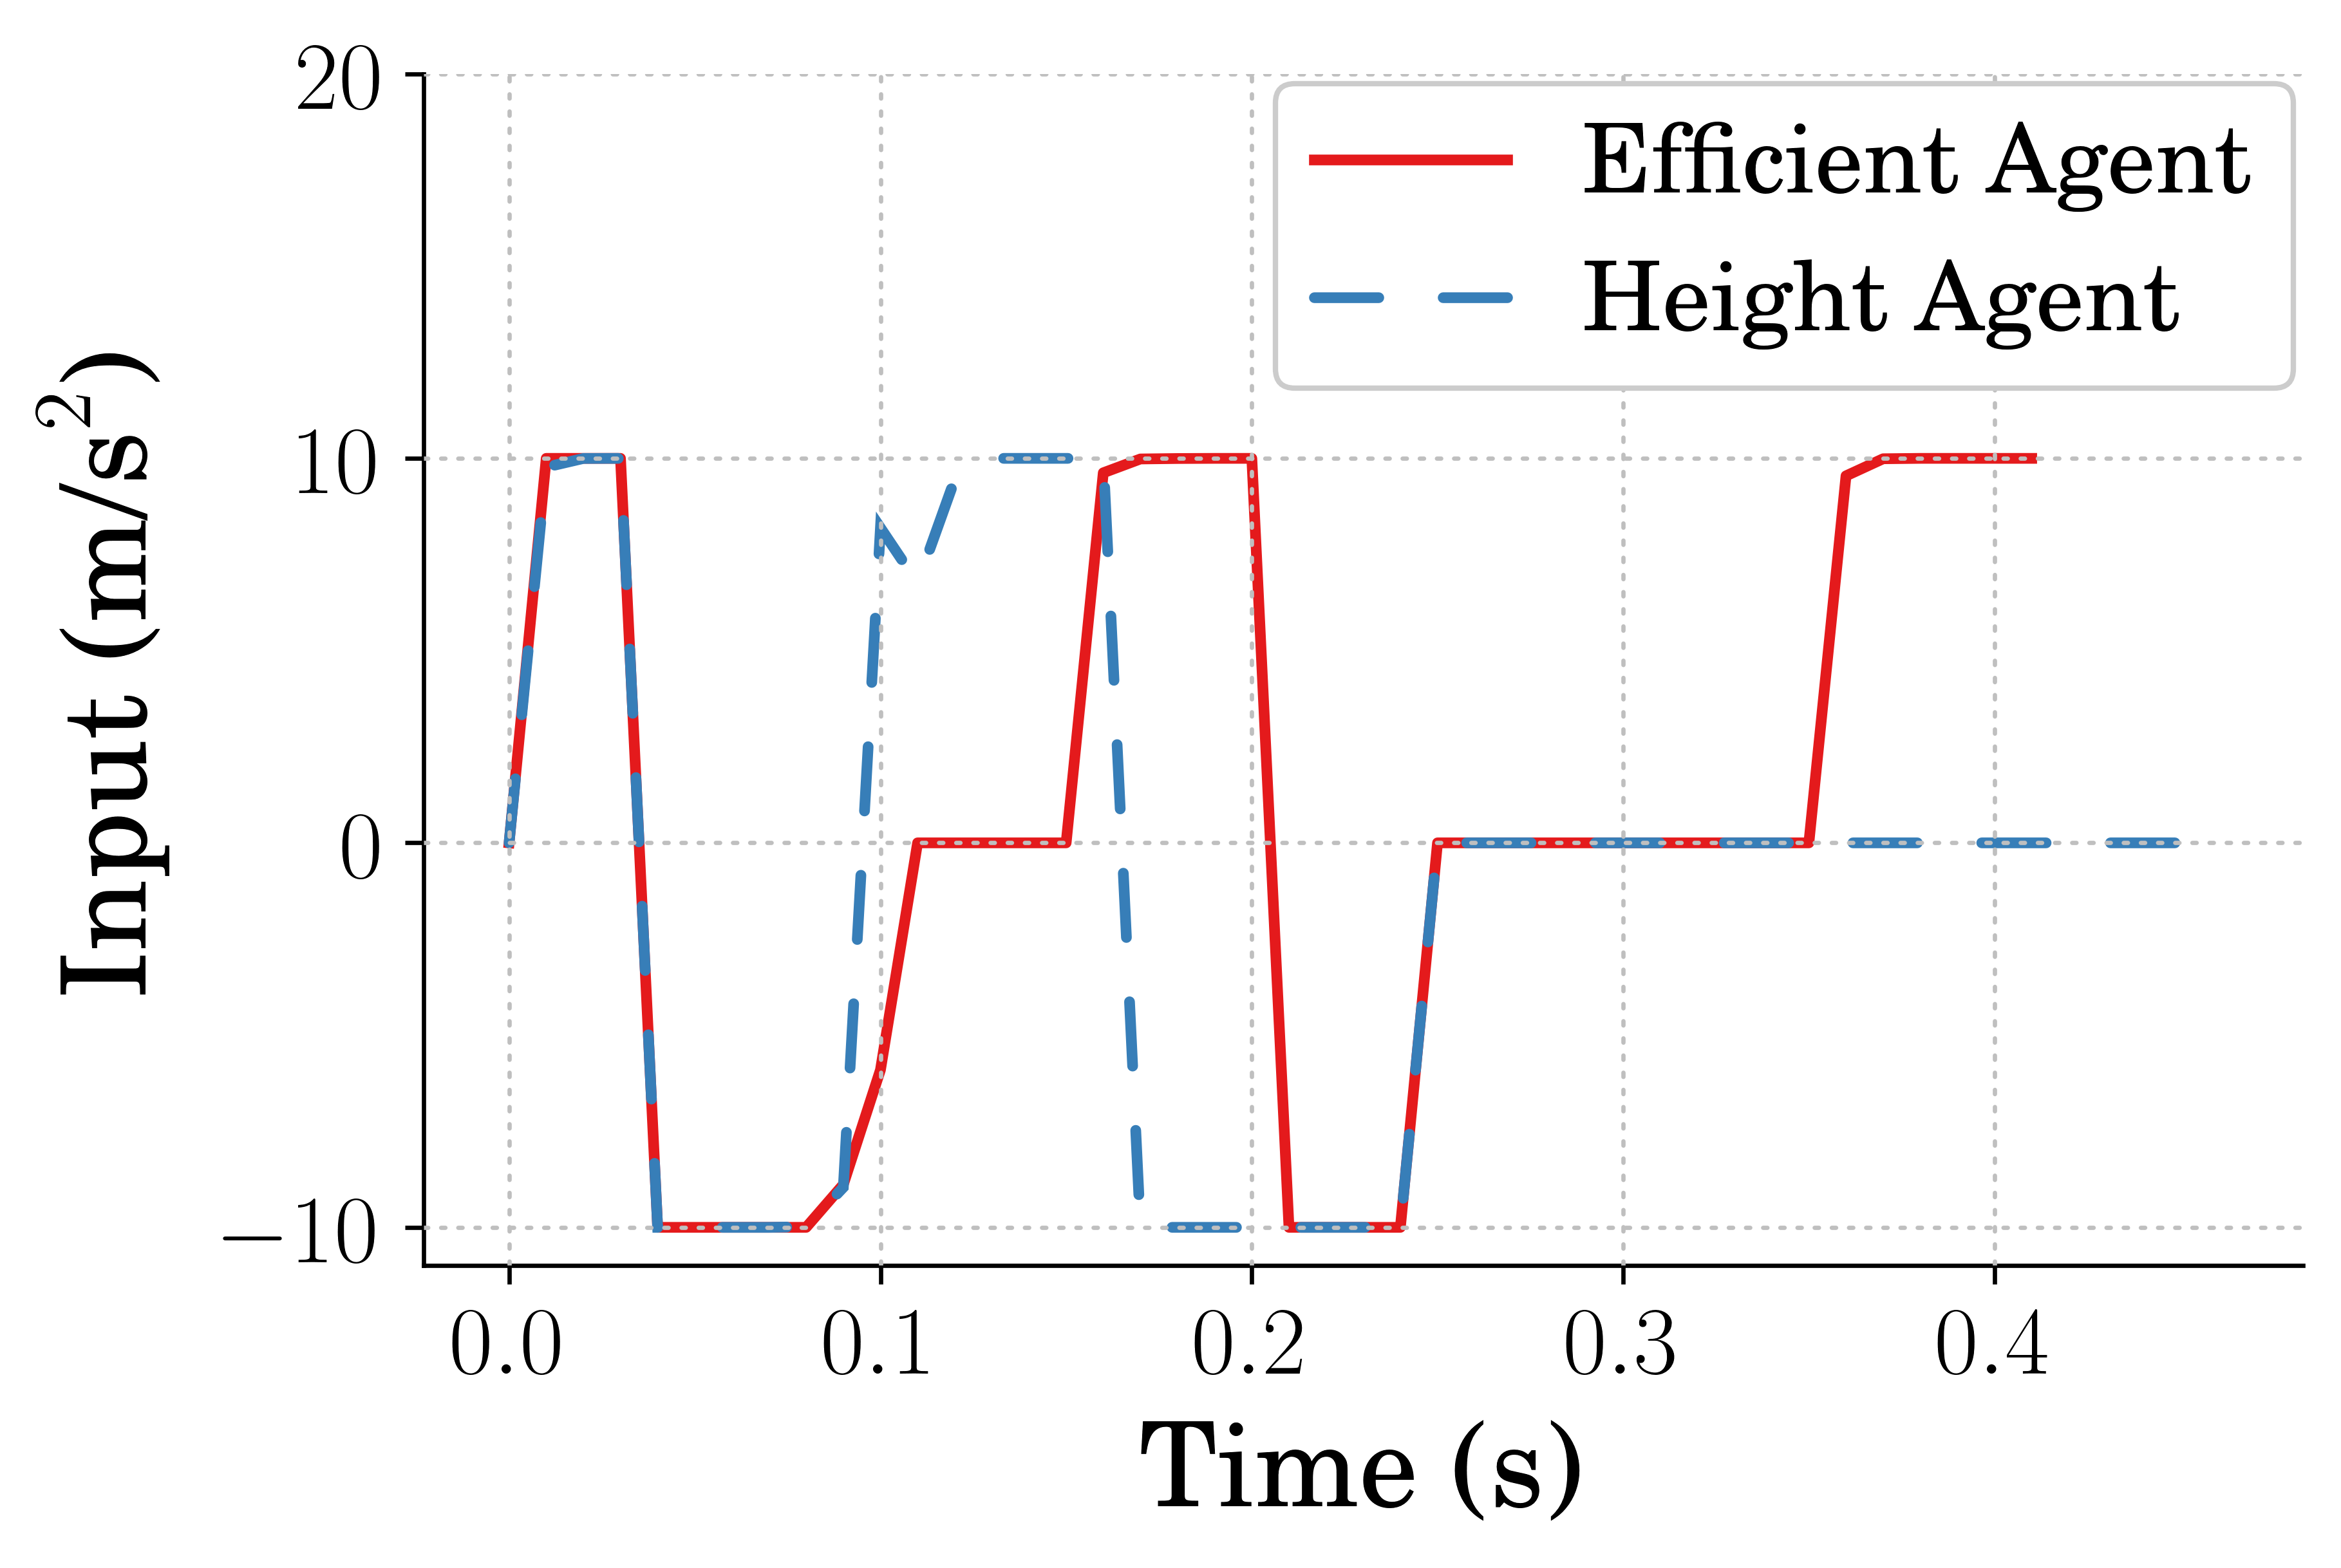
\includegraphics[width=\textwidth]{figures/Ch5/best_case/best_Stutter_Input_.png}  
    \caption{Best Case Efficient and High Jumping Inputs Learned}
    \label{fig:conc_best_input}
  \end{subfigure}
  \hfill
  \begin{subfigure}{.49\textwidth}
    \centering
    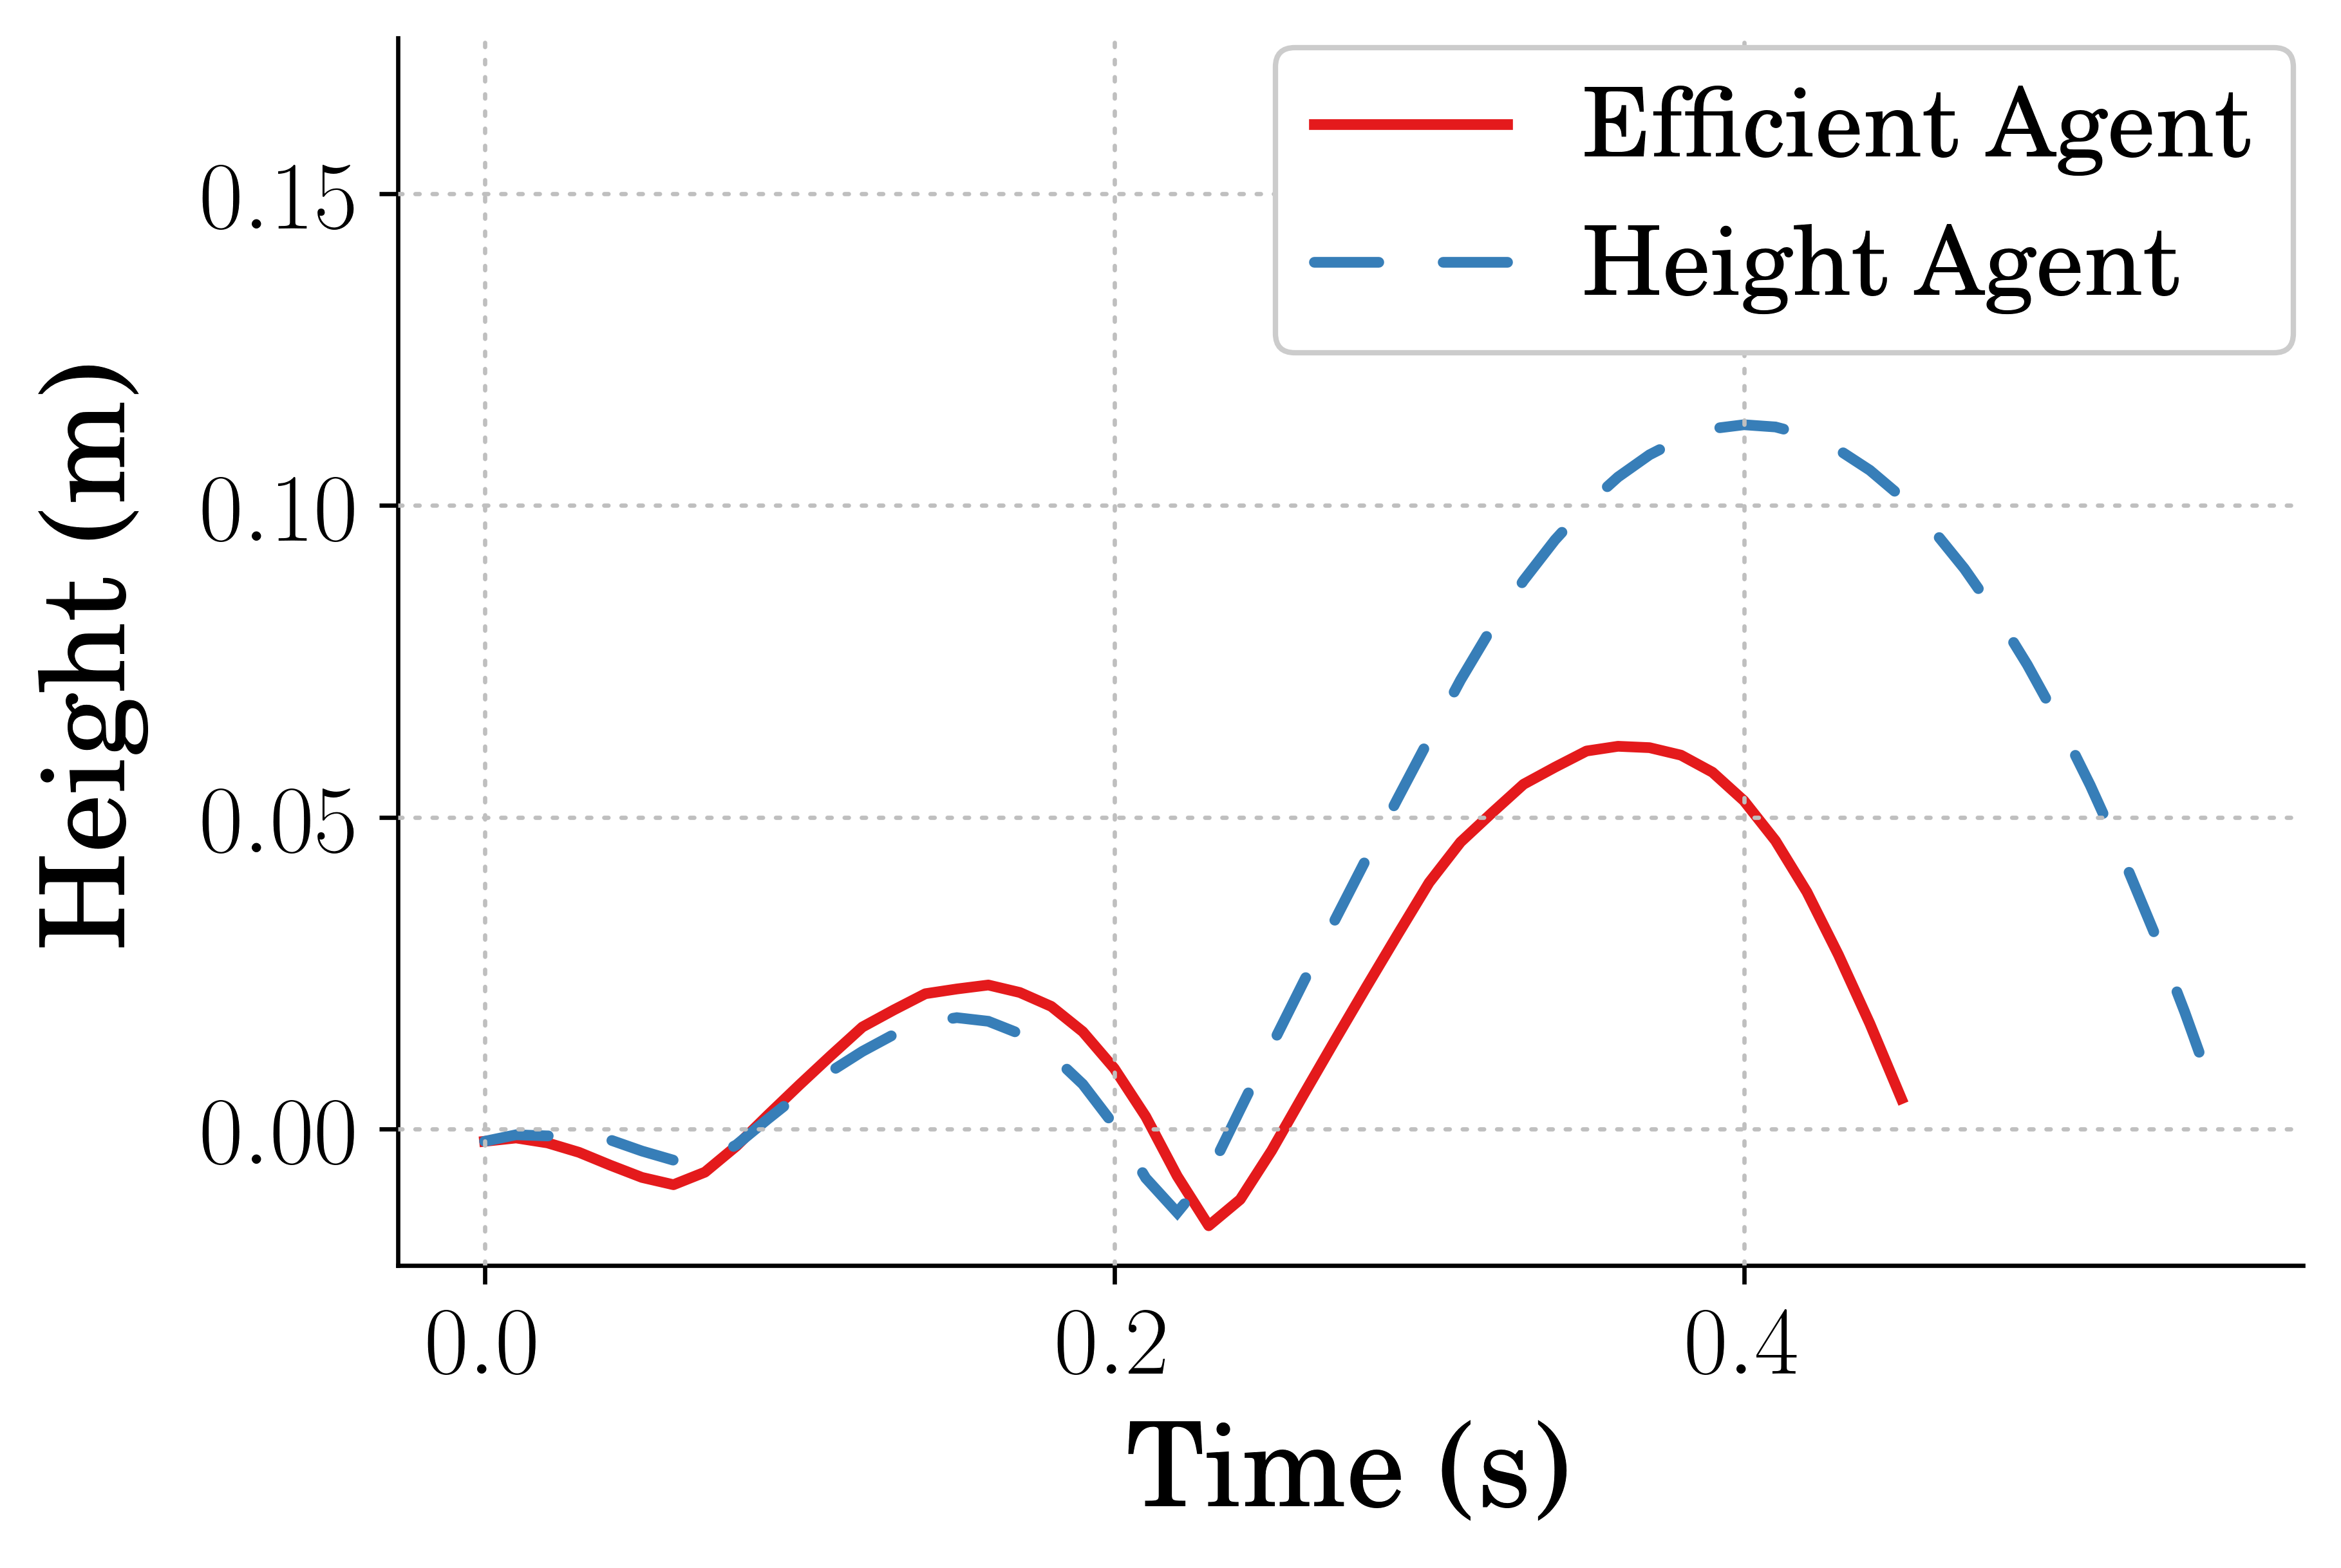
\includegraphics[width=\textwidth]{figures/Ch5/best_case/best_Stutter_RodPos_.png}  
    \caption{Best Case Efficient and High Jumping Heights}
    \label{fig:conc_best_rodpos}
  \end{subfigure}
   \caption{Best Case Performance for Concurrent Designs}
   \label{fig:conc_best_performance}
\end{figure}
% 
% Chapter 2:
% Max Efficient Height: 0.0607432013800848
% Max Height Height: 0.0915456169114579
% Percent Difference: 50.70923960466784
% Max Efficient Power Used: 17.93805315775764
% Max Height Power Used: 21.476888231927703
% Percent Difference: 19.72808890155189

% Concurrent Design
% Max Efficient Height: 0.061381406104032
% Max Height Height: 0.1129740794296378
% Percent Difference: 84.05260908843339
% Max Efficient Power Used: 27.127788774400898
% Max Height Power Used: 20.230354841387957
% Percent Difference: -25.42571379618561

%-----------------------------------------------------
\section{Conclusion}
A concurrent design architecture was defined and evaluated using the monopode jumping system discussed in Chapter~\ref{chapter2}. The architecture consists primarily of an inner and outer loop where the outer is defined to learn a control policy for an environment design that can be updated within the inner loop. The architecture was evaluated to generate an efficient and a high jumping, concurrently designed system and controller. Two methods for implementing the inner loop mechanical design update, being discrete and continuous, were discussed. The differences in learning and final concurrent design performance between these two methods were shown, and the use cases for each were discussed. In general, the continuous method showed more consistent learning across multiple instantiations of the concurrent design architecture, making it the more attractive option for the monopode system. Additionally, a new hyperparameter, being the rate at which the mechanical design is updated within the outer loop, was introduced. It was shown that changes to the update rate are of primary importance when altering the complexity of the control policy being trained. In general the concurrent design architecture struggled to find designs for the efficient jumping strategy due to the increased complexity of the control policy. As for the high jumping strategy, the designs found averaged higher performance than control policies trained on static mechanical designs like what shown in Chapter~\ref{chapter2}. Additionally, in the best case, the high jumping concurrent design also outperformed the best case of a policy trained on a static environment. It should be concluded then, that this type of architecture could be used where finding a concurrent design is of interest. However, the reward shape passed to the control policy should be considered carefully, as fragile policies become more fragile with dynamically changing environments.